\documentclass[a4paper,10pt]{article}
\usepackage[utf8]{inputenc}
\usepackage[spanish]{babel}
\usepackage[pdftex]{graphicx}

\makeindex

%opening
\title{\underline{\textbf{SuciOS}} \\ \small Standard Useless Command-line Interface Operating System}
\author{
Lezica, Santiago. (Leg. 49147).\\
Ballesty, Pablo Andrés. (Leg. 49359).\\
Pose, Jimena Belén. (Leg. 49015).\\
}
\date{Lunes 1 de Noviembre}

\begin{document}

\maketitle

\newpage
\tableofcontents

\newpage
\section{Introducción}
\subsection{Objetivo}
Realizar un programa que conmute diferentes procesos, asignándoles a cada 
uno un tiempo de ejecución. El multitasker no corre sobre ningún Sistema 
Operativo, se ubica en memoria utilizando un bootloader GRUB.


\subsection{Enunciado}
El trabajo consta de la realización de un Multitasker, cuyo objetivo es asignar
tiempo de ejecución a diferentes procesos en memoria. El sistema deberá ser
implementado para plataformas Intel de 32 bits, utilizando el procesador en
modo protegido. El multitasker debe ser preemptivo, es decir, cualquier tarea
puede ser desalojada del microprocesador. El encargado de administrar el CPU
es el scheduler el cual tomará como base de tiempo la interrupción de hardware
INT8 correspondiente al timer tick, para realizar la asignación de tiempo ( time
slot ).

\subsection{Contexto de tareas}
Cada grupo deberá elegir la forma en resguardar el contexto de cada tarea, las
opciones son: utilizar los TSS que provee el microprocesador Intel 386 o una
implementación propia de código.

\subsection{Scheduler}
El Multitasker deberá implementar 2 (dos) tipos de scheduling distintos. Al
menos uno de ellos deberá considerar la prioridad de los procesos para asignar
los slots de tiempo.

\subsection{Estados de procesos}
El sistema deberá estar programado de manera que se diferencien los estados
básicos de ”Corriendo”, ”Esperando” y ”Listo”. Por otra parte, cada proceso
deberá tener un valor de prioridad entre 0 y 4 que indique la importancia del
proceso. Además se deberá demostrar el funcionamiento de los mismos con
programas de prueba y se deberá poder corroborar el estado del proceso y el
porcentaje de procesador que esté ocupando con la ayuda del comando ”top”.
También deberá haber un comando kill que permita matar procesos en ejecución.
Tener en cuenta que kill debe matar también a todos los hijos de ese proceso.
Deberán desarrollar una system call (simil a yield) que fuerce al proceso actual
a ceder procesador.

\subsection{Terminales}
El usuario debe poder tener al menos 4 terminales distintas y alternar entre
ellas de manera similar a Linux.

\subsection{Intérprete de comandos}
El usuario debe poder ejecutar las diferentes tareas a través de comandos ingresados 
por teclado. La forma de los comandos quedan a elección del alumno.

\subsection{Procesos en background}
El sistema debe tener la posibilidad de correr los mismos procesos tanto en
foreground como en background. Para este último se deberá utilizar el caracter
``\&'' al igual que en UNIX.

\subsection{Administración de memoria}
El sistema debe tener un módulo de administración de memoria mediante paginación 
para los procesos, el mismo se encargará de lo siguiente:

\begin{itemize}
 \item Cada proceso tendrá su stack propio en una página, a la cual solamente él
	tendrá acceso. Cada proceso podrá leer y escribir libremente sobre esta
	página pero no páginas de otros procesos.      
 \item Los procesos no poseerán un heap propio, ya que están corriendo sobre la
	misma zona de datos del SO.
 \item Ningún proceso deberá leer o escribir directamente ninguna variable global
	del SO. En caso de que haya variables globales que estén pensadas para
	ser leidas por procesos usuario, deberán tener una función que las copie a
	una zona de heap propia al proceso, simulando un system call.
\end{itemize}

\subsection{Proveedor de Servicios}
Deberán implementar dos procesos proveedores de servicios, que estarán corriendo 
desde la inicialización del sistema. Estos procesos estarán constantemente
bloqueados esperando pedidos. Cuando algún proceso usuario requiera algún
servicio de algún servidor, lo llamará mediante un IPC (puede ser cualquiera,
incluso sencillo). El proceso servidor correrá con máxima prioridad y no podrá
ser interrumpido por otros procesos usuario, salvo que decida ceder procesador
voluntariamente.

\subsection{Programas de prueba}
Cada grupo deberá desarrollar tareas, que funcionarán como programas de
prueba, los mismos deberán demostrar vulnerabilidades y virtudes del trabajo,
y servirán para demostrar la implementación del TP.


\newpage


\section{Desarrollo}

\subsection{Llamadas al Sistema}
Todas las llamadas de sistema son accedidas a través del pseudo-objeto System. Por ejemplo:

System.name("my new task name");

A continuación sigue una guía detallada de todas las llamadas que ofrece SuciOS.

\subsubsection{Control de Tareas}

\begin{itemize}
 \item \textbf{int exec(program\_t program, char* line)}\\
    \noindent
    Crea una nueva tarea desde la función program, cuyo prototipo debe retornar integer y recibir como parámetro un char*.
    La línea line es pasada como parámetro a la tarea, que se coloca en la cola de tareas listas para ejecutarse.

 \item \textbf{int execb(program\_t program, char* line)}\\
    \noindent Como exec, pero ejecuta un proceso en background.

 \item \textbf{int yield()}\\
    \noindent Ofrece al sistema operativo la opción de desalojar inmediatamente a la tarea invocadora.

 \item \textbf{int wait()}\\
    \noindent Bloquea a la tarea invocadora hasta que uno de sus hijos finalice su ejecución.

 \item \textbf{int name(char* name)}\\
    \noindent Cambia el nombre de la tarea invocadora.

 \item \textbf{int getName(void* buf, int tid)}\\
    \noindent Recibe un task id, y escribe su nombre en el buffer buf. Cuídese que el buffer tenga MAX\_TASK\_NAME bytes. Retorna 0 si tiene éxito, -1 si ocurre un error.

\item \textbf{int getRMode(int tid)}\\
    \noindent Recibe un task id, y retorna su modo de ejecución FOREGROUND, o BACKGROUND.

 \item \textbf{int getStatus(int tid)}\\
    \noindent Recibe un task id, y retorna su estado de ejecución, o -1 en caso de error.

 \item \textbf{int getcpuc(int tid)}\\
    \noindent Recibe un task id, y retorna su porcentaje de consumo de cpu, o -1 en caso de error.

 \item \textbf{int getprio(int tid)}\\
    \noindent Recibe un task id, y retorna su prioridad, o -1 en caso de error.

 \item \textbf{int setPrio(int prio)}\\
    \noindent Cambia la prioridad del proceso invocador.

 \item \textbf{int getrank(int tid)}\\
    \noindent Recibe un task id, y retorna su rango (RANK\_NORMAL o RANK\_SERVER), o -1 en caso de error.

 \item \textbf{int setRank(int rank)}\\
    \noindent Cambia el rango del proceso invocador.

 \item \textbf{int gettid(char* name)}\\
    \noindent  Localiza una tarea llamada name, y retorna su tid, o -1 en caso de error. Si name es NULL, retorna el id de la tarea invocadora.

 \item \textbf{int nexttid(int* iter)}\\
    \noindent Recibe un puntero a entero en el espacio de programa, que se utilizará para controlar la iteración, y no necesita estar inicializado. Retorna el task id de alguna tarea en ejecución en su primera invocación, y uno diferente en cada invocación subsiguiente (siempre que se le pase como parámetro el mismo puntero a entero, y su contenido no se modifique por otra función). Es responsabilidad del llamador detener la iteración cuando le plazca: nexttid devolverá circularmente los ids de todas las tareas del sistema.

 \item \textbf{int kill(int tid)}\\
    \noindent Termina la tarea con el tid especificado.

 \item \textbf{int sleep(int n)}\\
    \noindent Duerme al proceso, evitando que el scheduler lo elija durante n pasadas.

\end{itemize}
 
\subsubsection{Conmutación entre Tareas}
\begin{itemize}
 \item \textbf{int send(int to, void* msg, int len)}\\
  \noindent Envía el mensaje contenido en el buffer msg, hasta el largo len, a la tarea con ID 'to'. La tarea bloquea hasta que el mensaje pueda ser enviado (lo cual requiere que el receptor invoque a System.recv()).
 \item \textbf{int recv()}\\
  \noindent Bloquea a la tarea invocadora hasta que un mensaje sea recibido, y devuelve la longitud del mensaje. Es la primera llamada al intentar recibir un mensaje.
 \item \textbf{int getmsg(void* buf, int len)}\\
  \noindent Transfiere un mensaje previamente recibido con System.recv() al espacio de proceso, en el buffer buf. Len debe ser igual al largo del mensaje informado por System.recv(), como medida de control. Debe llamarse inmediatamente después de recv(), sin recurrir a otras llamadas de sistema.
 \item \textbf{int clsmsg()}\\
  \noindent Destruye el mensaje almacenado por el kernel para este proceso. No es necesario llamarla entre mensajes, pero la tarea tiene la opción de hacerlo si desea.
\end{itemize}

\subsubsection{Entrada y Salida}
\begin{itemize}
 \item \textbf{int read(int dev, void* buf, int n)}\\
  \noindent Lee n bytes del dispositivo dev y los escribe en el buffer buf.
 \item \textbf{int seekr(int dev, int offset, int from)}\\
  \noindent Desplaza el puntero de lectura del dispositivo dev en offset bytes, desde una posición determinada por from (DEVICE\_START, DEVICE\_CURRENT o DEVICE\_END).
 \item \textbf{int seekw(int dev, int offset, int from)}\\
  \noindent Desplaza el puntero de escritura del dispositivo dev en offset bytes, desde una posición determinada por from (DEVICE\_START, DEVICE\_CURRENT o DEVICE\_END).
 \item \textbf{int tellr(int dev)}\\
  \noindent Retorna la posición del puntero de lectura del dispositivo dev.\\
 \item \textbf{int tellw(int dev)}
  \noindent Retorna la posición del puntero de escritura del dispositivo dev.
 \item \textbf{int write(int dev, void* buf, int n)}\\
  \noindent Escribe n bytes en el dispositivo dev, tomándolos de buf.
\end{itemize}

\subsection{Contexto de tareas}
Para guardar el contexto de las tareas se decidió realizar una implementación propia, 
la cual guarda en el stack de la tarea los valores necesarios. Al crear una tarea se crea
su stack, en el que se ubican (en el siguiente orden) una función de limpieza (para que 
cuando la tarea termine esta pueda liberar su stack y borrarse del vector de procesos), 
los eflags, el cs, el nuevo ip y los registros de uso general. \\
El cambio de contexto se lleva a cabo en la interrupción 20 (timer tick), por lo tanto 
en el manejador de esta, se busca la nueva tarea a correr y se hace apuntar el esp al stack 
de esta nueva tarea. Por último se levantan del stack los registros de uso general (los últimos 
empujados en la creación del mismo) y se hace un iret, que se encarga de levantar el ip, el cs 
y los eflags. En caso que la tarea haya terminado, el ip que levanta el iret es el de la tarea 
de limpieza.

\subsection{Scheduler}
Para este trabajo se implementaron dos scheduler, uno similar al \textit{Priority Round Robin} 
y otro similar al \textit{Lottery}, ambos consideran prioridades. En ambos casos se considera 
que si la tarea que estaba corriendo era un servidor no se le puede sacar el procesador y se 
la debe dejar corriendo. Por último, si no hay ninguna tarea lista para correr se retorna la 
tarea idle.

\subsubsection{Priority Round Robin}
En el caso del \textit{Priority Round Robin} se decidió darle mas prioridad a los procesos 
servidores, si bien estos corren con la máxima prioridad, se los prioriza por encima de procesos 
con la misma prioridad que no sean servidores. En caso de no haber ningún proceso servidor listo 
para correr se corre el resto de los procesos en orden, asignándoles un tiempo de ejecución según 
su prioridad.

\subsubsection{Lottery}
Para el \textit{Lottery} se decidió armar una función que devuelva un número random entre 0 y 100, basándose 
en la cantidad de ticks del procesador. El siguiente proceso a correr se elige según lo que devuelva esta función, 
si devuelve un valor entre 0 y 49 se le da la oportunidad de correr a un proceso con prioridad 0, 
si devuelve un valor entre 50 y 69 se busca uno de prioridad 1, entre 70 y 84 uno de prioridad 2, entre 85 y 94 
uno de prioridad 3, y por último, entre 95 y 100 uno de prioridad 4.\\
En caso que no se encuentre un proceso con la prioridad deseada, se busca otro pasando desde prioridad 0 hasta 
prioridad 4. Si bien esto no es muy eficiente (se puede llegar a estar recorriendo el vector de prioridades muchas 
veces) se consideró que si hay alguna tarea lista para correr el scheduler no debe devolver el proceso idle, por lo 
tanto si no encuentra la tarea con la prioridad determinada por la función random debe buscar otra con la mayor 
prioridad posible.

\subsection{Estados de procesos}
Se decidió crear los siguientes estados:

\begin{itemize}
 \item STATUS\_READY - La tarea está lista para correr.
 \item STATUS\_WAITING - La tarea está bloqueada esperando.
 \item STATUS\_DEAD - La tarea está marcada como muerta.
 \item STATUS\_RUNNING - La tarea está corriendo.
 \item STATUS\_WAITING\_RECV - La tarea está esperando a recibir un mensaje.
 \item STATUS\_WAITING\_SEND - La tarea está esperando a enviar un mensaje.
 \item STATUS\_WAITING\_SLEEP - La tarea está durmiendo.
\end{itemize}

En cuanto a las prioridades se tienen las siguientes:

\begin{itemize}
 \item PRIORITY\_MAX - Prioridad 0
 \item PRIORITY\_HIGH - Prioridad 1
 \item PRIORITY\_MEDIUM - Prioridad 2
 \item PRIORITY\_LOW - Prioridad 3
 \item PRIORITY\_MIN - Prioridad 4
\end{itemize}


Se implementó el comando top que muestra la infromación y el porcentaje 
de procesador que ocupa cada proceso. Para demostrar el funcionamiento del 
sistema operativo se implementaron programas de prueba detallados más adelante.\\

El comando kill termina la tarea indicada por el id pasado como parámetro, sacándola del vector de procesos y 
liberando su stack. Por otro lado marca con STATUS\_DEAD a todos sus procesos hijos 
con el fin de que en la próxima ejecución cada hijo termine con sí mismo y sus
respectivos hijos. \\

Se implementó el yield haciendo que el proceso se ponga en STATUS\_READY y llamando 
al scheduler para que una nueva tarea pueda ser elegida.

\subsection{Terminales}
En el trabajo de arquitectura, el kernel poseía varias estructuras denominadas ``devices'' en las cuales se 
especificaban la dirección de memoria, un offset de escritura, un offset de lectura, y el tamaño de memoria que
utilizaba un device. Para el diseño de las terminales, se agregó un device denominado ``DEVICE\_TTY'' en el cual
se alojaba la terminal en la que corría el proceso que tenía dominio del procesador, este device funciona como el
``output''. El DEVICE\_TTY arranca inicializado sobre la dirección de memoria de video, permitiendo
al kernel imprimir mensajes de inicialización. Para el ``input'' el kernel ya tenía el DEVICE\_KEYBOARD, el cual fue utilizado
para enrutar la entrada a la terminal activa. En la función de ``scheduling'' se hizo que al realizarse un cambio de tarea,
se haga el correspondiente switch de DEVICE\_TTY, en cambio para la entrada, se hizo que esta siempre escriba en la terminal
activa, y siempre lea de la terminal que le pertenece al proceso. De esta manera las funciones getchar() y putchar() funcionaban
con su correspondiente terminal. Para mantener la terminal activa sobre la pantalla, por motivos de comodidad, se decidió hacer
un update de pantalla desde la interrupción del timer tick, con un REFRESH\_RATE definido.\\
\noindent A continuación se presenta un gráfico esquemático con la terminal TTY0 activa, suponiendo que hay un proceso corriendo sobre ella.

\begin{center}
 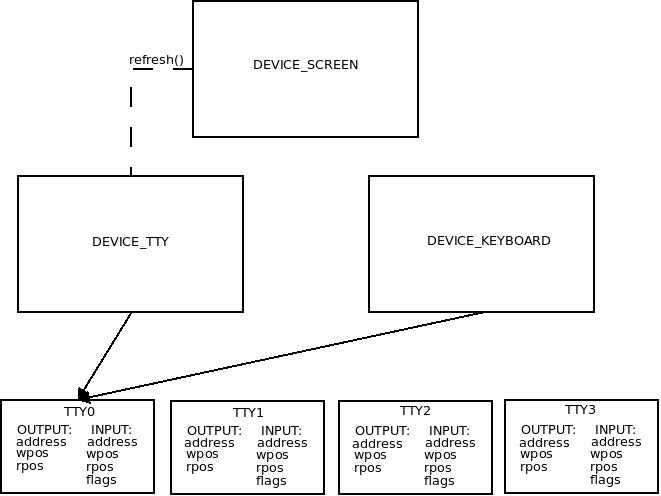
\includegraphics[scale=0.45]{./terminales.jpeg}
 % terminales.jpeg: 661x496 pixel, 72dpi, 23.32x17.50 cm, bb=0 0 661 496
\end{center}


\subsection{Intérprete de comandos}
Para el intérprete de comandos se reutilizó el desarrollado en arquitectura, es simplemente una función llamada \textbf{shell()}, la
cual posee un buffer interno para ir recibiendo el comando, y una vez que se presiona \textit{Enter} se lo parsea y se lo ejecuta en caso
de existir. Cabe aclarar que la función shell() es totalmente independiente de la terminal, al comenzar el kernel se crean 4 procesos
corriendo ésta función sobre cada terminal.


\subsection{Procesos en background}
Cuando se crean tareas se pide un runningMode el cual podrá ser RUNNING\_FRONT y RUNNING\_BACK, cuando un proceso tiene como runningMode 
RUNNING\_BACK sus read a DEVICE\_KEYBOARD no surgen efecto, por lo tanto queda aislado del ``input''.


\subsection{Administración de memoria}
Al arrancar el Sistem operativo, se obtiene la cantidad de memoria existente, ésta se le pasa a la función Paging.start(), la cual se encarga de
armar la estructura de directorios y tablas para paginar la memoria, setear el registro CR3 y activar la paginación en CR0. Por motivos
de complejidad se decidió hacer ``Indentity Mapping'' en toda la memoria, es decir, que las direcciones físicas y lógicas coinciden.
Los primeros 4MB de memoria fueron destinados exclusivamente al Kernel, alojando en su última página el directorio, y detrás de éste un bitmap para
el manejo de páginas libres. Los próximos 4MB fueron destinados para alojar las tablas, en este espacio hay lugar para alojar todas las tablas necesarias
para paginar 4GB aunque se utilizarán solamente las necesarias.\\
Se desarrolló la función \_sys\_malloc la cuál retorna un bloque de páginas contiguas necesarias para alojar la cantidad de memoria pedida. La función malloc
que se le brinda al usuario, buscará espacio libre en los bloques ya pedidos por la tarea que realiza el malloc, y si no encuentra, pedirá un nuevo bloque
al sistema y lo adherirá a la tarea.\\
\noindent A continuación se presenta un gráfico esquemático, en el cual el usuario hace por primera vez malloc y aloja datos, luego hace otro y los datos se
alojan en el mismo bloque, y luego hace otra vez malloc y se genera un nuevo bloque. Cabe aclarar que los free que realiza el usuario no hacen nada, cuando
el proceso muere se eliminan todos los bloques generados por el mismo.

\begin{center}
 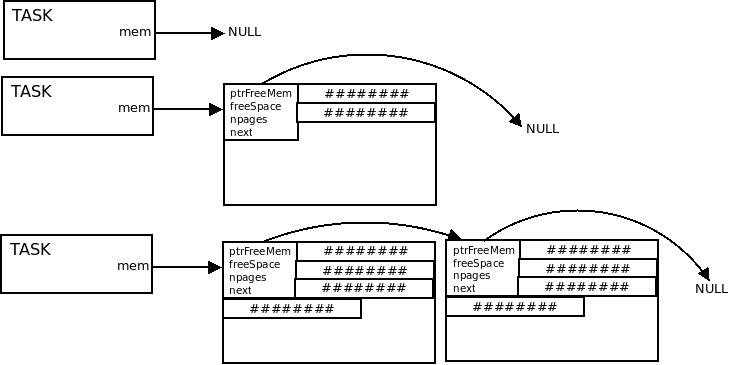
\includegraphics[scale=0.45]{./malloc.jpeg}
 % terminales.jpeg: 661x496 pixel, 72dpi, 23.32x17.50 cm, bb=0 0 661 496
\end{center}

\subsection{Proveedor de Servicios}

\subsection{Programas de prueba}
\begin{itemize}
 \item \textbf{demo\_malloc}\\
      \noindent Este comando ejecuta una función la cual realiza 1000 mallocs de size 100 bytes, logrando hacer un testing suficiente para ver
      que se adhieren nuevos bloques a la memoria de la tarea. Si éste se corre varias veces, se nota que al haber terminado una tarea, se liberan los
      bloques que esta tomo, y la nueva ejecución toma ese mismo espacio liberado.
 \item \textbf{doNothing}\\
      \noindent Este comando ejecuta una función que crea una tarea que a su vez crea otra, para armar una rama de tareas y poder hacer un correcto testing del
	kill.
 \item \textbf{echoserver}\\
      \noindent Este comando ejecuta una función para el testing del IPC.
 \item \textbf{doGetChar} \\
      \noindent Este comando ejecuta una función que realiza un getchar, y termina cuando el usuario presiona una tecla. Esto nos permite hacer un testing
	  de tareas corriendo en background. Si ejecutamos este comando en background, el programa queda colgado en el getchar(), y deberemos matarlo con
	  kill.
 \item \textbf{testFree}\\
      \noindent A último momento se agregó este comando para demostrar que salta el Page Fault, si queremos acceder a memoria no paginada.
\end{itemize}


\newpage
\section{Conclusiones}
Luego del desarrollo del trabajo práctico especial llegamos a las siguientes conclusiones:
\begin{itemize}
 \item Entendimos qué era realmente un sistema operativo con multitasking, y la complejidad que resulta desarrollarlo.
 \item Comprendimos las ventajas de un sistema con memoria paginada, y la seguridad que brinda esta característica. Aunque
    lograr un eficiente y seguro manejo de memoria es muy complejo.
 \item Haber logrado un acercamiento a un sistema operativo multitasking con manejo de tareas, terminales, procesos en background, fue un gran
      esfuerzo, pero luego de este gran esfuerzo nos resulta muy gratificante poder jugar creando procesos, matarlos, ejecutarlos en background, etc.
 \item Viendo lo que nos costó hacer un mínimo sistema operativo, vemos la real magnitud de trabajo que tienen encima los sitemas operativos modernos,
      que cotidianamete utilizamos.

 \item Si bien uno de los grandes problemas de los sistemas operativos es el sincronismo de tareas, no nos resultó un gran desafío
      este tema gracias a una buena organización.
\end{itemize}

\bigskip
\end{document}
